\documentclass[10pt, a5paper]{article}
\usepackage{pdfpages}
\usepackage{parallel}
\usepackage[T2A]{fontenc}
\usepackage{ucs}
\usepackage[utf8x]{inputenc}
\usepackage[polish,english,russian]{babel}
\usepackage{hyperref}
\usepackage{rotating}
\usepackage[inner=2cm,top=1.8cm,outer=2cm,bottom=2.3cm,nohead]{geometry}
\usepackage{listings}
\usepackage{graphicx}
\usepackage{wrapfig}
\usepackage{longtable}
\usepackage{indentfirst}
\usepackage{array}
\newcolumntype{P}[1]{>{\raggedright\arraybackslash}p{#1}}
\frenchspacing
\usepackage{fixltx2e} %text sub- and superscripts
\usepackage{icomma} % коскі ў матэматычным рэжыме
\PreloadUnicodePage{4}

\newcommand{\longpage}{\enlargethispage{\baselineskip}}
\newcommand{\shortpage}{\enlargethispage{-\baselineskip}}

\def\switchlang#1{\expandafter\csname switchlang#1\endcsname}
\def\switchlangbe{
\let\saverefname=\refname%
\def\refname{Літаратура}%
\def\figurename{Іл.}%
}
\def\switchlangen{
\let\saverefname=\refname%
\def\refname{References}%
\def\figurename{Fig.}%
}
\def\switchlangru{
\let\saverefname=\refname%
\let\savefigurename=\figurename%
\def\refname{Литература}%
\def\figurename{Рис.}%
}

\hyphenation{admi-ni-stra-tive}
\hyphenation{ex-pe-ri-ence}
\hyphenation{fle-xi-bi-li-ty}
\hyphenation{Py-thon}
\hyphenation{ma-the-ma-ti-cal}
\hyphenation{re-ported}
\hyphenation{imp-le-menta-tions}
\hyphenation{pro-vides}
\hyphenation{en-gi-neering}
\hyphenation{com-pa-ti-bi-li-ty}
\hyphenation{im-pos-sible}
\hyphenation{desk-top}
\hyphenation{elec-tro-nic}
\hyphenation{com-pa-ny}
\hyphenation{de-ve-lop-ment}
\hyphenation{de-ve-loping}
\hyphenation{de-ve-lop}
\hyphenation{da-ta-ba-se}
\hyphenation{plat-forms}
\hyphenation{or-ga-ni-za-tion}
\hyphenation{pro-gramming}
\hyphenation{in-stru-ments}
\hyphenation{Li-nux}
\hyphenation{sour-ce}
\hyphenation{en-vi-ron-ment}
\hyphenation{Te-le-pathy}
\hyphenation{Li-nux-ov-ka}
\hyphenation{Open-BSD}
\hyphenation{Free-BSD}
\hyphenation{men-ti-on-ed}
\hyphenation{app-li-ca-tion}

\def\progref!#1!{\texttt{#1}}
\renewcommand{\arraystretch}{2} %Іначай формулы ў матрыцы зліпаюцца з лініямі
\usepackage{array}

\def\interview #1 (#2), #3, #4, #5\par{

\section[#1, #3, #4]{#1 -- #3, #4}
\def\qname{LVEE}
\def\aname{#1}
\def\q ##1\par{{\noindent \bf \qname: ##1 }\par}
\def\a{{\noindent \bf \aname: } \def\qname{L}\def\aname{#2}}
}

\def\interview* #1 (#2), #3, #4, #5\par{

\section*{#1\\{\small\rm #3, #4. #5}}

\def\qname{LVEE}
\def\aname{#1}
\def\q ##1\par{{\noindent \bf \qname: ##1 }\par}
\def\a{{\noindent \bf \aname: } \def\qname{L}\def\aname{#2}}
}

\switchlang{en}
\begin{document}
\title{Using eye trackers for the oculographic research in GNU/Linux}
\author{Dmitriy Kostiuk, Anastasia Markina, Brest, Belarus\footnote{\url{asyamarkina2@gmail.com}, \url {https://lvee.org/ru/abstracts/322}}}
\maketitle
\begin{abstract}
The analysis of oculography is presented taking into account the physiological and psychological characteristics of a person, as well as possible ways of using modern oculographic devices (eye trackers) to track the user's gaze direction in GNU/Linux. The overview of the features and performance of both software and hardware implementations is given. An experimental scheme used by the authors to study user interaction with graphical applications in GNU/Linux is discussed. The limitations and interpretation specifics are discussed.
\end{abstract}
When interacting with modern software, vision plays the role of the main, and in some cases, the only channel for perceiving information. At the same time, the clear and detailed vision provided by the central part of the retina covers an extremely small area, but half of the information processing is dedicated to it. Accordingly, detailed information is \linebreak obtained using visual sampling and scanning \cite{bib1}.

Oculographic research involves the analysis of the gaze movement and the areas of visual focalization on which the gaze is concentrated. Its application to assess the effectiveness of human-machine interaction can be divided into three categories \cite{bib2}:

\begin{itemize}
  \item identification of sources of difficulties (time-consuming form filling, etc.), in particular, related to the noticeability of elements, points of focus, mental stress and distractions;
  \item identification of specifics of user behavior (visual search strategies, reading and scanning patterns);
  \item comparison of several design decisions in conjunction with other types of testing (questionnaire, another biometric assessment).
\end{itemize}

Modern eye trackers typically use digital cameras that record the user's eye movements. The tracker is mounted on the user's head or is stationary fixed in the field of view.

Developers who wish to perform the oculographic testing of GNU/ Linux software have several options. The most budget option is the face and eye recognition using a webcam. This approach is implemented in such free projects as eviacam, TrackEye, WebGazer.js. They can be used to track gaze \cite{bib3}, but the result is very limited due to the webcam: it has a low frame rate and effective gaze positioning accuracy (half the resolution of the camera), and it is also difficult to recognize head rotation. Professional IT trackers, designed for research laboratories with a large budget (for some of them there are drivers for Linux) are on the opposite end of the scale. And there is a compromise solution, eye trackers that are targeted at the entertainment area but have accuracy sufficient for research tasks [4, 5]. We used together with GNU/Linux the eye trackers of this compromised category, produced by Tobii.

Tobii eye trackers are divided into the expensive Tobii Pro \linebreak professional series and consumer segment devices, for which the \linebreak manufacturer offers two types of SDKs: a low-level Stream Engine (declared to support Linux) and a higher-level Core SDK. We have tested two eye trackers, Tobii REX и Tobii EyeX. The alpha version of Stream Engine for Linux appeared only in 2018, and before there was a low-level Gaze SDK for Linux, which is currently not provided by the company.

\begin{center}
\begin{figure}[h!]
  \centering
  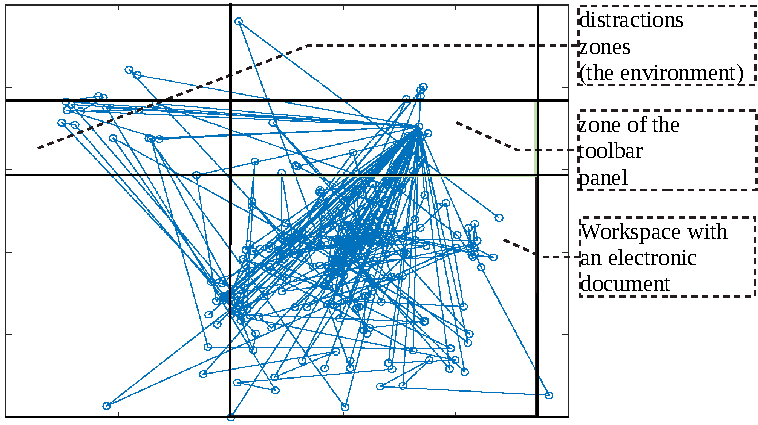
\includegraphics[width=10cm]{Markina1}
  \caption{User's gaze fixations when working with the application}	
  \label{markina:fig1}
\end{figure}
\end{center}

As a result of work, the eye tracker produces an array of coordinates corresponding to the position of the gaze at various points in time. Central vision provides information about the fine details of the image, but covers a relatively small part of the field of view; as a result, information is received using visual sampling, and peripheral vision indicates the next point of focus \cite{bib5}. The gaze moves with rapid leaps (saccades) with short pauses between them (fixations). So, when working with text, 7–9 letters are read in one saccade, and the fixation time is about 250 milliseconds, but the perception extends to twice as many letters due to peripheral vision \cite{bib7}. However, in the study of eye \linebreak movements, only central vision is recorded, and peripheral is not taken into account.

Visualization of the results of eye-tracking provides two options:

\begin{itemize}
  \item building a heat map, highlighting parts of the screen depending on the intensity of fixing the gaze;
  \item time-lapse mapping.
\end{itemize}

In both cases, the map is superimposed on the image of the user's working screen. When processing in GNU/Linux, it is convenient to use GNU Octave with a two-dimensional nuclear density estimation function to create heat maps by coordinates \cite{bib8}, and in case of a gaze map, one can just draw a graph in Graphviz, or also in Octave (see Fig. \ref{markina:fig1}, which illustrates the user’s work with a typical office application).

The parameters of descriptive statistics characterizing the shift of the distribution center are also informative when evaluating the results of the experiment (Fig. \ref{markina:fig2}): it is advisable, first of all, to select the middle region through which the gaze passes, calculate the median, the average value of the coordinates of the point where the gaze was fixed, and also determine the point at which the user most often focused his eyes, using mode.

If necessary, the percentage of eye fixations on individual functional parts of the application window (for example, the toolbar) and eye fixations outside the window (distraction area) can serve as simple numerical estimates of human-machine interactions obtained based on eye tracker data.

It is also necessary to take into account that there are physiological limitations due to which this technique cannot be applied: for example, nystagmus, which is characterized by involuntary eye movements with a high frequency, as a result of which the brain receives a fuzzy image of the object, and the eye tracker is not able to catch eye gaze.

\begin{center}
\begin{figure}[h!]
  \centering
  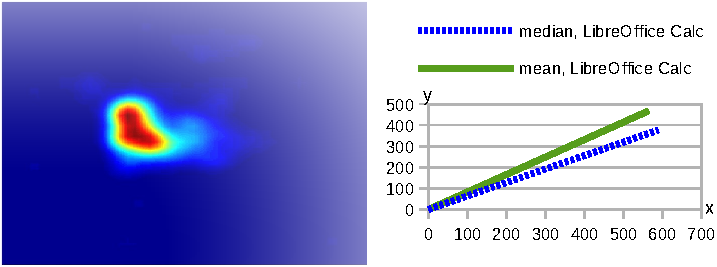
\includegraphics[width=10cm]{Markina2}
  \caption{Typical heatmap for gaze focalization (left) and shift of the distribution center of the sample (right) by the example of the table processor usage}	
  \label{markina:fig2}
\end{figure}
\end{center}


\begin{thebibliography}{9}
\bibitem{bib1} Titz J., Scholz A., Sedlmeier P. Comparing eye trackers by correlating their eye-metric data // Behav. Res., 2017.\url{https://www.ncbi.nlm.nih.gov/pubmed/28879442}
\bibitem{bib2} Дубицкий А., Костюк Д., Маркина А., Фомин С. Применение айтрекеров для юзабилити-исследований ПО в GNU/Linux // Четырнадцатая конференция разработчиков свободных программ: тезисы докладов – Калуга, 22–24 сентября 2017 г. – М. : Базальт СПО, 2017. – С. 36–41.
\bibitem{bib3} Semmelmann K., Weigelt S. Online webcam-based eye tracking in cognitive science: A first look // Behav. Res. 2017. \url{http://rdcu.be/tjzF.23}
\bibitem{bib4} Gibaldi A. et al. Evaluation of the Tobii EyeX Eye tracking controller and Matlab toolkit for research // Behav. Res. V. 49, 2017. P.923–946.
\bibitem{bib5} Ludwig C.J.H., Davies J.R., Eckstein M.P. Foveal Analysis and Peripheral Selection during Active Visual Sampling. // Proc. of the National Academy of Sciences of the USA. V. 111(2), 2014. P. E291–E299.
\bibitem{bib6} Goodman K.S. On Reading. / Portsmouth, NH: Heinemann, 1996. 152 p.
\bibitem{bib7} Ulloa A. Auto Heat Mapper. \url{https://github.com/aulloa/Auto_Heat_Mapper}
\end{thebibliography}
\end{document}
